\documentclass{article}

\usepackage{natbib}
\usepackage{algorithm}
\usepackage{algorithmic}
\usepackage{amsmath}
\usepackage{geometry}
\usepackage{verbatim}
\usepackage{tabularx}
\usepackage{graphicx}
\usepackage{amsfonts} % just for the indicator variable \mathbb{I}

\title{Elo-R Competition Rating System}
\author{Aram Ebtekar}
\date{December 2015 (revised on May 22, 2020)}

\begin{document}
\maketitle

\section{Introduction}

This paper describes the Elo-R rating system, designed for use in programming competitions. The ``R" in the name may stand for ``Ranked", as it operates on game outcomes given as a rank-ordered list of players; or it may stand for ``Robust", as its ratings are robust to outlier performances, like someone having a bad day in which their Internet connection died.

Competitions, in the form of sports, games and examinations, have been with us since antiquity. Whether for entertainment, training, or selection for a particular role, contestants and spectators alike are interested in estimating the relative skills of contestants. Skills are easiest to compare when there is a standard quantifiable objective, such as a score on a standardized test or a completion time in a race.  However, most team sports, as well as games such as chess, have no such measure. Instead, a good player is simply one who can frequently win against other good players.

The Elo rating system assigns a quantitative measure of skill to each player. For example, an average player may be rated 1500, while a top player may exceed 2500. The scale is arbitrary, but can be used to rank players relative to one another. The odds of any one player winning against another may be estimated from the difference in their ratings. The famous Elo system, and variants such as Glicko \cite{glicko}, provide useful formulas for updating ratings of players who compete 1v1 against one another, resulting in a winner and a loser. These algorithms have some nice properties: they are fairly simple, fast, and only modify the ratings of the two participating players.

Now let's consider a general setting in which a typical contest has much more than two participants. An arbitrary number of players compete simultaneously at a task. Rather than producing just a winner and a loser, the contest ranks its participants 1st place, 2nd, 3rd, and so on. This description fits popular programming competition websites such as Codeforces \cite{Codeforces} and TopCoder \cite{TopCoder}, each of which has tens of thousands of rated members from across the globe. Each publishes its own rating system, but without much theoretical justification to accompany the derivations.

We build Elo-R upon a more rigorous probabilistic model, mirroring the Bayesian development of the Glicko system. In doing so, we inherit its nice properties in practice, resolving known issues with the Codeforces and TopCoder systems. Compared with these systems, it achieves faster convergence and robustness against unusual performances. Issues specific to Codeforces than we improve upon are the overall spread of ratings, inter-division boundary artifacts, and inflation (TODO: cite, and quantify this with tests). An issue specific to TopCoder that we eliminate completely is non-monotonicity: simply put, there are cases in which improving a member's past performance would actually decrease their TopCoder rating, and vice-versa \cite{forivsektheoretical}.

Furthermore, Elo-R retains simplicity and efficiency on par with the other systems. To demonstrate this, I provide a very efficient parallel implementation that can process the entire history of rated competitions hosted by Codeforces on a modest quad-core laptop within 30 minutes. It is implemented entirely within the safe subset of Rust using the Rayon crate; hence, the Rust compiler verifies that it contains no data races.

This paper is organized as follows: in section 2, we develop a Bayesian model for the competitions. Rating updates are phrased as a latent skill estimation problem, which is naturally divided into two phases. Sections 3 and 4 describe each of these phases in turn, and supplement the derivations with some intuitive interpretations. Then in section 5, we discuss some ways to model uncertainty, in a manner analogous to the Glicko system. In section 6, we discuss some properties of the Elo-R system in comparison with the Codeforces and TopCoder systems. Finally, section 7 presents the conclusions of this work.

\section{Bayesian Model}

Now we describe the setting formally. A series of competitive \textbf{rounds}, indexed by $t=1,2,3,\ldots$, take place sequentially in time. The participants of a round $t$ are a subset of all the \textbf{players}, which are indexed by $i$. At time $t$, player $i$ has latent \textbf{skill} $s_{i,t}$, which we seek to estimate from a history of observable \textbf{evidence} $e_1,\ldots,e_t$ produced by the rounds $1,\ldots,t$.

In Bayesian fashion, we start with a prior belief distribution on $s_{i,t}$ immediately preceding round $t$, taking into account all of the rounds $1,2,\ldots,t-1$. In section 5, we'll see how the prior distribution at round $t$ differs from the posterior distribution at round $t-1$, but for now this distinction can be ignored.

In any case, our main task is to combine the prior belief with the evidence $e_t$ to obtain a posterior belief. This will serve as the basis for a post-round \textbf{rating}, defined to be the \textbf{maximum a posteriori} (MAP) estimate of $s_{i,t}$. That is,

\[r_{i,t} = \arg\max_{s_{i,t}} f(s_{i,t} \mid e_1,\ldots,e_t) = \arg\max_{s_{i,t}} f(s_i \mid e_1,\ldots,e_{t-1}) \Pr(e_t \mid s_i)\]

where $f(s_{i,t} \mid e_1,\ldots,e_t)$ is the probability density function (p.d.f.) corresponding to our posterior belief on player $i$'s latent skill given the history of evidence. Here we used Bayes' rule to write the posterior p.d.f. as proportional to the product of the prior p.d.f. and the evidence probability.

Let's simplify the notation. Since the pre-round evidence $e_1,\ldots,e_{t-1}$ is common to both the prior and posterior beliefs, we treat them as understood and explicitly write only the new evidence $e_t$. This leaves $t$ as the only round subscript, so we omit that as well. With these changes, the post-round rating can be re-written more simply as

\[r_i = \arg\max_{s_i} f(s_i \mid e) = \arg\max_{s_i} f(s_i) \Pr(e \mid s_i)\]

We assume the evidence $e$ is produced from each round in the following generative fashion: each participant randomly draws their performance $p_i$ in the round independently from a logistic distribution centered at $s_i$, with a variance $\gamma_i^2$ that may depend on characteristics of the match $t$ (whose subscript we continue to omit) and player $i$.

While the variables $s_i$ and $p_i$ are hidden, we assume that player $i$ outranks player $j$ (written $i \succ j$) in the round if, and only if, $p_i > p_j$, and that we observe the complete relative rankings. In other words, the observable evidence $e$ consists of a total order on the set of participants.

Due to this important modeling assumption, the method is best-suited for competitions in which the most pertinent information is round rankings. Note that, in the programming contest setting, this means we discard specific information about player scores, which are difficult to model and depend heavily on the specifics of the problem set. This method would be ill-suited to model, for instance, track races, where a runner's absolute time is more informative than relative rankings. On the other hand, it may be very well-suited to obstacle-course races, if each round consists of novel obstacles that make the absolute times hard to interpret.

Strictly speaking, ties have probability zero of occurring in our model. Assuming that ties are relatively infrequent in programming contests, they can be handled with a special modification that we'll describe later, essentially treating them as half a win and half a loss.

\begin{center} 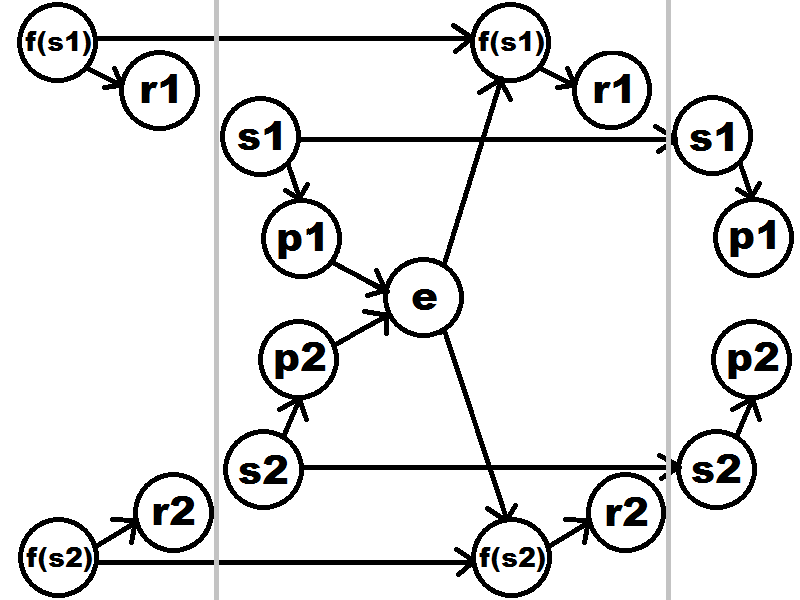
\includegraphics[scale=0.35]{../images/HMMlabeled.png} \end{center}

In order to absorb $e$ into our posterior, a few approximations are in order. First, we assume the number of participants is so large that we are able to compute the performances exactly. Mathematically, this means $\Pr(e \mid p_i)$ is proportional to a delta ``function" concentrated at the correct value of $p_i$. Hence, using Bayes' rule again,

\begin{align*}
f(s_i\mid e)
&\propto f(s_i)\Pr(e\mid s_i)
\\&= f(s_i)\int \Pr(e\mid p_i)f(p_i\mid s_i)\,dp_i
\\&\propto f(s_i)f(p_i\mid s_i)
\end{align*}

where the constants of proportionality depend on $e$ but not on $s_i$.

This suggests a natural two-phase update algorithm for each player $i$. In phase one, we estimate the MAP of $p_i$ given $e$. This estimate has very low error in the limit of very many participants, so we can take the MAP of $p_i$ to be its true value. In phase two, we update the posterior according to the above expression, and compute the new rating $r_i$ as the MAP of $s_i$ given $e$.

Note that, since the $p_i$ are assumed to be computed exactly, there is never a reason to retroactively update past estimates of performance. It follows that a round's non-participating players have posterior skill distribution identical to their prior; in particular, their ratings do not change.

\section{Performance Estimation}

Since our assumptions imply the posterior on $p_i$ to be narrowly concentrated, the MAP estimate is as good as any. Thus, we seek to maximize

\[f(p_i\mid e) \propto f(p_i) \Pr(e\mid p_i)\]

In the prior distribution, $p_i = s_i + (p_i-s_i)$ is a sum of two independent random variables. $s_i$ has the prior distribution, whose mode is the pre-match rating $r'_i$; let $\sigma_i^2$ be its variance. The other term $p_i-s_i$ is a zero-centered logistic random variable with variance $\gamma_i^2$.

The sum of two normal random variables is another normal variable whose mean is the sum of the component means. Inspired by this fact, we make another approximation: although neither $s_i$ nor $p_i-s_i$ are normal, we treat their sum $p_i$ as a logistic random variable centered at $r'_i$. By independence of its two components, $p_i$ has variance $\delta_i^2 = \gamma_i^2 + \sigma_i^2$.

We'll adopt the convention that any symbol that represents a standard deviation is multiplied by $\frac{\sqrt{12}}{\pi}\approx 1.1$ when drawn with an upper-bar. For example, $\bar\delta_i = \frac{\sqrt{12}}{\pi} \delta_i$. In terms of $\bar\delta_i$, the logistic p.d.f. takes a convenient form:

\[f(p_i) \approx \frac { 2e^{2(p_i-r'_i)/\bar\delta_i} } { \bar\delta_i\left(1 + e^{2(p_i-r'_i)/\bar\delta_i} \right)^2}\]

Since we are working in the limit of a large number of players, we have sufficient evidence to determine $p_i$ even after ignoring relations like $j \succ k$ which don't include $i$. Thus, we can imagine $e$ to be the evidence consisting solely of, for each $j\ne i$, whether $j \succ i$ or $j \prec i$. Taking $p_i$ as fixed in the following probability expressions, using the logistic cumulative density function (c.d.f.), and ignoring constants of proportionality that depend on $e$ but not on $p_i$:

\begin{align*}
\Pr(e\mid p_i)
&= \prod_{j \succ i} \Pr(p_j > p_i) \prod_{j \prec i} \Pr(p_j < p_i)
\\&\approx \prod_{j \succ i} \frac {1} {1 + e^{2(p_i-r'_j)/\bar\delta_j}} \prod_{j \prec i} \frac {e^{2(p_i-r'_j)/\bar\delta_j}} {1 + e^{2(p_i-r'_j)/\bar\delta_j}}
\\&\propto \frac {e^{2p_i\sum_{j\prec i}1/\bar\delta_j}} {\prod_{j\neq i} 1 + e^{2(p_i-r'_j)/\bar\delta_j}}
\end{align*}

Taking logarithms, there exist constants $C$ and $C'$ such that
\begin{align*}
C + \ln f(p_i\mid e)
&= C' + \ln f(p_i) + \ln \Pr(e\mid p_i)
\\&\approx \frac{2}{\bar\delta_i} (p_i-r'_i) - 2\ln\left(1 + e^{2(p_i-r'_i)/\bar\delta_i} \right) + 2p_i\sum_{j\prec i} \frac{1}{\bar\delta_j} - \sum_{j\neq i} \ln\left(1 + e^{2(p_i-r'_j)/\bar\delta_j}\right)
\end{align*}

To maximize this expression, differentiate it w.r.t. $p_i$ and set the result to zero:
\begin{align*}
0 &= \frac{2}{\bar\delta_i}\left(1 - \frac {2e^{2(p_i-r'_i)/\bar\delta_i}} {1 + e^{2(p_i-r'_i)/\bar\delta_i}} \right)
+ \sum_{j\neq i}\frac{2}{\bar\delta_j}\left(\mathbb{I}(j\prec i) - \frac {e^{2(p_i-r'_j)/\bar\delta_j}} {1 + e^{2(p_i-r'_j)/\bar\delta_j}} \right)
\\&= \sum_{j\preceq i}\frac{2}{\bar\delta_j}\left(\frac {1} {1 + e^{2(p_i-r'_j)/\bar\delta_j}} \right)
- \sum_{j\succeq i}\frac{2}{\bar\delta_j}\left(\frac {e^{2(p_i-r'_j)/\bar\delta_j}} {1 + e^{2(p_i-r'_j)/\bar\delta_j}} \right)
\\&= -\left( \sum_{j\preceq i}\frac{1}{\bar\delta_j}\left( \tanh\frac {p_i - r'_j} {\bar\delta_j} - 1 \right)
+ \sum_{j\succeq i}\frac{1}{\bar\delta_j}\left( \tanh\frac {p_i - r'_j} {\bar\delta_j} + 1 \right) \right)
\end{align*}

By monotonicity of the $\tanh$ function, we can solve for $p_i$ by a simple binary search. If faster convergence is desired, Newton's method can be used: since $\frac{d}{dx}\tanh(x) = 1 - \tanh^2(x)$, a Newton step is very efficient, requiring no more hyperbolic function evaluations than a binary search step.

On the second line, the terms in parentheses can be thought of as a measure of surprise at the outcomes between $i$ and $j$: they are the probability of the outcomes opposite to what actually occurred, when the performance of player $i$ is fixed to $p_i$. In addition to the actual outcomes which come from $e$, the prior hallucinates two regularizing outcomes: one in which player $i$ wins against itself, and one in which player $i$ loses against itself. This regularization prevents the first- and last-place players from achieving $p_i = \pm\infty$. By choosing $p_i$ such that the sum equals zero, we are effectively saying that the total surprise from wins should equal the total surprise from losses.

Here's another intuitive interpretation: if the $\delta_j$s are all equal, this amounts to finding the performance level $p_i$ at which one's expected rank would equal player $i$'s actual rank, after accounting for the regularizing clones of player $i$. With unequal $\delta_j$s, this interpretation can be extended to a weighted ranking in which player $j$ counts $\frac{1}{\delta_j}$ times.

Now we see an easy way to handle ties: simply treat them as half a win and half a loss. Since the above expression subtracts 1 for each win and adds 1 for each loss, averaging the two yields an offset of 0 for ties. It's a hack, but an elegant one!

\section{Belief Update}

With $p_i$ in hand, we are ready for the second phase of the update! Recall that we seek to maximize

\[f(s_i\mid e) \propto f(s_i)f(p_i\mid s_i)\]

Ignoring for now the distinction between the posterior at round $t-1$ and the prior at round $t$, we see that each round multiplies our belief p.d.f. by a logistic factor and a normalizing constant. Thus, our belief will always consist of a product of p.d.f.s.

Let's be a tad more general here and allow the belief to be any normalized product of normal and logistic p.d.f.s. The normal p.d.f.s can be composed into a single normal with mean and variance $(\mu_0, \tau_0^2)$. Let $R_i$ be the set of rounds in which player $i$ has participated, each contributing a logistic factor with parameters $(\mu_k, \tau_k^2)$ for $k\in R_i\cap \{1,\ldots,t\}$. Naturally, the new factor from round $t$ will have $\mu_t = p_{i,t}$ and $\tau_t = \gamma_{i,t}$. Again defining $\bar\tau_k = \frac{\sqrt{12}}{\pi} \tau_k$,

\begin{align*}
f(s_i\mid e)
&\propto e^{-(s_i-\mu_0)^2/\tau_0^2} \prod_k \frac { e^{2(s_i-\mu_k)/\bar\tau_k} } { \left(1 + e^{2(s_i-\mu_k)/\bar\tau_k} \right)^2 }
\\&= e^{-(s_i-\mu_0)^2/\tau_0^2} \prod_k \frac { 1 } { \left( e^{-(s_i-\mu_k)/\bar\tau_k} + e^{(s_i-\mu_k)/\bar\tau_k} \right)^2 }
\\&= e^{-(s_i-\mu_0)^2/\tau_0^2} \prod_k \frac { 1 } { \left( 2\cosh\frac{s_i-\mu_k} {\bar\tau_k} \right)^2 }
\end{align*}

Hence, there exists a constant $C$ such that

\[C + \frac 1 2 \ln f(s_i \mid e) = -\frac{(s_i-\mu_0)^2}{2\tau_0^2} - \sum_k \ln\left( \cosh\frac{s_i-\mu_k}{\bar\tau_k} \right)\]

To maximize this expression, differentiate w.r.t. $s_i$ and set the result to zero:

\begin{align*}
0 &= -\left( \frac{s_i-\mu_0}{\tau_0^2} + \sum_k \frac{1}{\bar\tau_k} \tanh \frac {s_i-\mu_k} {\bar\tau_k} \right)
\end{align*}

Similar to the performance computation in the previous section, here we have a monotonic function of $s_i$. To compute the post-round rating $r_i = \arg\max_{s_i} f(s_i \mid e)$, we may use binary search or Newton's method.

This time, the intuitive interpretation comes from the pre-differentiated expression. By flipping the minus signs, we obtain a minimization objective with one term corresponding to each p.d.f. factor: the normal p.d.f. becomes a familiar $L^2$ penalty that pushes $s_i$ towards $\mu_0$. The logistic p.d.f.s are more interesting: they too are penalties that push $s_i$ towards $\mu_k$; however, instead of a simple squared error, we have the logarithm of a hyperbolic cosine!

At small scales (that is, when $|s_i-\mu_k| \ll \tau_k$), it acts like an $L^2$ penalty. However, at large scales (when $|s_i-\mu_k| \gg \tau_k$), it acts like an $L^1$ penalty! It's well-known that minimizing a sum of $L^2$ terms pushes the argument towards a weighted mean, while minimizing a sum of $L^1$ terms pushes the argument towards a weighted median. The latter feature is due to the thicker tails of the logistic distribution, compared to the normal. In practice, it makes our rating algorithm robust to outlier performances that are far below or above the rest. This seems reasonable, as contest performances have empirically been seen to have thick tails, more like the logistic than the normal (TODO citation).

Note that when the rating is a weighted mean, it's possible to compute the posterior rating as a function of only the prior rating, prior weight, and the current round's performance and weight. This is no longer possible when using $L^1$ or $\ln\cosh$ penalties. Naively, it appears this method must remember the entire history of past performances: certainly, the latest rating alone is insufficient.

Luckily, it's possible to sustain negligible loss of precision while retaining only a bounded history length per player, thus keeping the time and memory overhead to within a constant factor. We'll see in the next section that old performances will eventually have very large $\tau_k$. Since the $\tanh$ function behaves like the identity in the limit of large $\tau_k$, it's clear from the above expression that old logistic factors will come to resemble normal factors.

As a final matter, we estimate the variance $\sigma_i^2$ of the posterior distribution on $s_i$. While this is intractable for general products of p.d.f.s, we take advantage of our observation that logistic factors behave in the limit like normal factors. Thus, we make an approximation based on a formula that holds for products of normal p.d.f.s:

\[\frac{1}{\bar\sigma_i^2} = \frac{1}{\tau_0^2} + \sum_k \frac{1}{\bar\tau_k^2}\]

\section{Uncertainty}

So far, we've shown how to go from prior to posterior belief in any given round. Two gaps remain: the ``newbie prior" on the skill of a player who has never competed, and the update from posterior in one round to prior in the next.

The newbie prior is fairly simple: for Codeforces, I chose a normal distribution with mean 1500 and standard deviation 350. The normal's thin tails discourage the granting of extreme ratings until sufficient evidence is gathered to justify it. To more strongly discourage premature assignment of extreme ratings, a smaller standard deviation can be used.

The remaining gap concerns the update that goes on between rounds, while a player is absent from competition. There are many ways to approach this, depending on what characteristics are desired of the rating system. Typically, we don't want to adjust the mean $r$ of a player's skill distribution, but we may want to increase the uncertainty $\sigma$ to account for the fact that a player may have improved or worsened during the time in which we haven't seen them compete. Thus, we might have $\sigma^2$ increase with time at a constant rate, as if the player's skill were being slowly and randomly perturbed by a process of Brownian motion. In this model, a long-inactive player's skill has to potential to change considerably upon their return. In a system that implements such Brownian noise, if we report the lower-bound estimate $r-2\sigma$ instead of $r$, we would find that ratings gradually decay, favoring active players and gradually diminishing inactive ones.

For Codeforces, we prefer to preserve the ratings of inactive players. Furthermore, we consider it likely that players who compete frequently would develop much faster than those who are inactive. Thus, it makes sense to increase uncertainty on a per-round basis rather than on a continuous per-time basis. Only on rounds in which a player competes, their pre-round $\sigma^2$ is increased by a noise term $\eta^2$. Post-round, their $\sigma^2$ is decreased according to the performance uncertainty, which I set to a constant $\bar\gamma = 250$ (though it's worth considering smaller $\gamma$ for longer contests, which are likely to be more informative). Over sufficiently many rounds, this process will eventually approach the limit $\sigma^*$ given by the fixpoint equation:

\begin{align}
\frac{1}{\sigma^{*2}} &= \frac{1}{\sigma^{*2} + \eta^2} + \frac{1}{\gamma^2}
\\ \text{Setting }\bar\sigma^*=100\text{, I derived }\bar\eta^2 &= \frac{1}{1/\bar\sigma^{*2} - 1/\bar\gamma^2} - \bar\sigma^{*2} \approx 43.64^2
\end{align}

Note that if the prior uncertainty is set to $\sigma^*$, we obtain a system in which the inter-round noise $\eta$ exactly compensates for the round information $\gamma$, and so $\sigma$ stays constant, similar to traditional Elo. However, I like to use a higher prior uncertainty and report $\mu-2(\bar\sigma-\bar\sigma^*)$ as a player's public rating. Without Brownian time-based noise, this doesn't cause rating decay; instead, its effect is to encourage beginners by presenting ratings that initially rise from the bottom rather than decline from the middle. Since players start with a low published rating instead of an average one, even middle ratings can be considered an achievement.

A simple way to increase the uncertainty from $\sigma^2$ to $\sigma^2 + \eta^2$ between rounds is to multiply the variance of each factor in the posterior skill distribution by the same value $1 + \frac{\eta^2}{\sigma^2}$. Once again, this can be rigorously justified by appealing to the limit of normal priors: adding a zero-mean noise term should not affect the mean of our belief distribution, and this is ensured by keeping the ratio of weights contributing to the belief distribution constant.  Intuitively, if we think of each factor as a ``measurement" of the current skill $s_{i,t}$, then the noise operation simply reduces our confidence in outdated measurements.

As promised in the previous section, now we see that each $\tau_k$ in the belief distribution will increase exponentially with additional rounds. Pretty soon, any plausible skill level $s_i$ will fall squarely within the regime where $|s_i-\mu_k| \ll \tau_k$. As a result, the older logistic factors can safely be absorbed into the normal factor.

The parameter and belief initializations are summarized in Algorithm \ref{alg:init}, while the actual Elo-R update is summarized in Algorithm \ref{alg:update}. Upper-bars are not drawn, but should be taken as implicit on all variances aside from the normal prior. By working with these modified variances, the algorithm avoids needing to compute the factor $\frac{\sqrt{12}}{\pi}$.

\begin{algorithm}
\caption{$init()$}
\label{alg:init}
\begin{algorithmic}
\STATE $\sigma^* := 100$
\STATE $\gamma := 250$
\STATE $\eta := \sqrt{1 / \left( 1/\sigma^{*2} - 1/\gamma^2 \right) - \sigma^{*2}}$
\FORALL{players $i$}
\STATE $\mu_i$ := queue with [$1500$]
\STATE $\tau_i$ := queue with [$350$]
\STATE $r_i := 1500$
\STATE $\sigma_i := 350$
\ENDFOR
\end{algorithmic}
\end{algorithm}

\begin{algorithm}
\caption{$update()$}
\label{alg:update}
\begin{algorithmic}
\FORALL{match participants $i$ in parallel}
\FORALL{$k$}
\STATE $\tau_{i,k} := \tau_{i,k} \sqrt{1 + \eta^2/\sigma_i^2}$
\ENDFOR
\STATE $\delta_i := \sqrt{\sigma_i^2 + \eta^2 + \gamma^2}$
\STATE Make $r'_i,\delta_i$ accessible in the next parallel loop
\ENDFOR
\FORALL{match participants $i$ in parallel}
\STATE $p_i := $ SOLVE $\sum_{j\preceq i}\frac{1}{\delta_j}\left( \tanh\frac {p_i - r'_j} {\delta_j} - 1 \right) + \sum_{j\succeq i}\frac{1}{\delta_j}\left( \tanh\frac {p_i - r'_j} {\delta_j} + 1 \right) = 0$
\IF{len(belief) $\ge$ MAX\_HISTORY}
\STATE $\mu_{i,0} := \left( \tau_{i,0}^2 \mu_{i,1} + \tau_{i,1}^2 \mu_{i,0} \right) / \left( \tau_{i,0}^2 + \tau_{i,1}^2 \right)$
\STATE $\tau_{i,0} := \tau_{i,0}\tau_{i,1} / \sqrt{ \tau_{i,0}^2 + \tau_{i,1}^2 }$
\STATE $\mu_i$.pop()
\STATE $\tau_i$.pop()
\ENDIF
\STATE $\mu_i$.push($p_i$)
\STATE $\tau_i$.push($\gamma$)
\STATE $r_i := $ SOLVE $\frac{r_i-\mu_{i,0}}{\tau_{i,0}^2} + \sum_{k\ge 1} \frac{1}{\tau_{i,k}} \tanh \frac {r_i-\mu_{i,k}} {\tau_{i,k}} = 0$
\STATE $\sigma_i := 1 / \sqrt{\sum_k 1/\tau_{i,k}^2}$
\ENDFOR
\end{algorithmic}
\end{algorithm}

\section{Properties (TODO: everything from here onwards needs serious rewriting. Please stop reading!)}

First, we discuss some properties that Elo-R has in common with the published systems of Codeforces and TopCoder, as well as the classics Elo and Glicko. All of these systems propagate belief changes forward in time, never backward. This approach is simple, efficient, and has the benefit of never retroactively changing ratings from the past, nor the ratings of player who are not actively competing. Elo-R and Glicko converge to the right results a bit faster than the others, by including an uncertainty parameter that starts high for new players.

The two-phase approach of Elo-R is a bit unique, in that it's not memoryless (unless the memory is set to merge all the way down to a length of 1). Rating changes depend not only on the current rating and uncertainty, but on a list of recent performance values. Thus, we cannot make the same guarantees as Codeforces \cite{Codeforces}. This is the price of a robust system: it's impossible to identify and eliminate outliers if we don't remember their values! Nevertheless, we have some analoguous guarantees:
\begin{itemize}
\item The rating is a monotonic function of the list of past performances. Thus, unlike on Topcoder \cite{forivsektheoretical}, a situation will never arise where we would wish to have scored less.
\item If you swap the order of two performances in the list, the rating goes up if the better performance moves forward in time, and down if the better performance moves backward. This follows from the fact that newer performances have smaller uncertainty, since uncertainties don't depend on the value of any performance.
\item The performance $p_i$ is measured in the same units as rating and has the property that, within a given contest, a higher ranking contestant always has higher $p_i$ than a lower ranking one. In case of ties, the contestant with higher rating $r_i$ also has (slightly) higher $p_i$.
\end{itemize}

The code and ratings of real Codeforces members as computed by Elo-R are available at https://github.com/EbTech/EloR. Original Codeforces ratings are at http://codeforces.com/ratings. One striking difference is massive inflation in the Codeforces system. Gennady Korotkevich, best known by his competitive programming handle ``tourist", has been the reigning world champion for years. Toward the end of 2011, his rating reached a new ceiling of about 2700 according to both systems. However, as of this writing, his rating on Elo-R has increased by about 300 additional points, while on Codeforces it increased by almost 900. To get a sense of the magnitude of this change, 900 points is the difference between an average member and a Grandmaster! Indeed, most of the variance in the Codeforces system is concentrated at the top, with much smaller rating differences between beginner and intermediate members. This is caused by certain ad hoc elements of the system that are not founded on any rigorous model.

This paper will not evaluate the predictive accuracy of Elo-R; my experience with it suggests it does better than the other local methods listed above, but it is possible to do better with global methods. It's difficult to do a fair evaluation because it's not clear what exactly some of these models are trying to predict, besides the qualitative assertion that players with higher ratings should win more often. For example, Elo-R might be judged on the log-likelihood of observed match results, according to its own belief model. However, the joint likelihood is difficult to compute, and many of the other systems lack a corresponding belief model. One reasonable approach would be to approximate the likelihood as we did when estimating $p_i$, and use cross-validation to optimize the parameters of each rating system according to this criterion. Such evaluations will remain open to future investigation. Instead, let's focus on a unique feature of Elo-R that's absent in the Codeforces system, and arguably in TopCoder as well.

\subsection{Robustness}

Imagine a player who performs very consistently over a long period of time, repeatedly achieving $p_i = 1000$ until convergence. Now, perhaps as a result of attending an intensive training camp in Petrozavodsk, their skill changes dramatically. From this point on, they consistently achieve $p_i = 3000$.

How does each rating system respond to the first such surprise occurrence? Elo-R treats the new result as a fluke, an outlier that ought to be ignored. The player gains 48 points; as a result of the parameters we set, this is the maximum possible for an experienced player as $p_i \rightarrow \infty$. In practice, ratings may change by more than 48, as the maximum depends on existing fluctuations in their history; here we're looking at the extreme example of a player with a history of always performing at exactly $p_i = 1000$.

\begin{center} 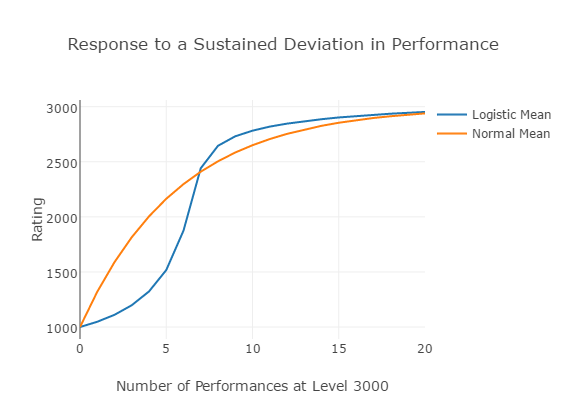
\includegraphics[scale=0.5]{../images/ResponsePlot.png} \end{center}

Had we tried to perform outlier reduction in a memoryless fashion, we would continue to increase the rating by 48 per match, oblivious to the possibility that the player truly did experience a sudden improvement. In Elo-R, the outlier status of a performance is treated as tentative. If later matches support the hypothesis of having improved, the rating will increase by an additional 63 points, followed by over 100 points in each of the third and following matches, as plotted by the blue curve above.

After six consecutive matches with $p_i = 3000$, the rating is 1875 and very unstable (even though $\sigma_i$ is unchanged!). The system is no longer sure which to trust: the extensive history at level 1000, or the smaller number of recent matches at level 3000. Depending on what comes next, the player's rating can very quickly fall toward 1000 or rise toward 3000. However, note that in either case, the change will not overshoot, say to 5000, unless enough new evidence is accumulated at that level. As the $p_i=3000$ streak continues, the seventh match on the blue curve jumps by a whopping 566 points. As the player's rating converges to 3000, the old $p_i = 1000$ data acquires outlier status, thus speeding convergence.

In contrast, while a system such as Codeforces does not compute $p_i$ values in quite in the same way, we can obtain a good approximation by removing outlier reduction from Elo-R, effectively treating the performances to be averaged as normal instead of logistic measurements. This makes the system effectively memoryless, since it turns out that each match simply moves the rating about 16\% closer to the new $p_i$ value, independent of the history. With this change, we obtain the orange curve, which jumps a whopping 320 points at the very first performance. Indeed, there is no limit: if you could find players whose ratings are extremely high, and beat them even once, your rating would take arbitrarily large leaps.

Note that this is not quite true of TopCoder, which incorporates a hack that caps the maximum rating change: if TopCoder's update formula demands too large a change, the cap kicks in. In contrast, Elo-R's cap is a natural and smooth consequence of its update formula and is sensitive to whether a change is charting new territory, or merely confirming a plausible hypothesis. TopCoder does attempt to make the magnitude of its updates sensitive to the amount of fluctuation in a player's history, using a volatility measure, but this measure does not account for the direction of the changes, resulting in the non-monotonicity flaw mentioned above.

Notwithstanding arguments that a high rating ought to properly be earned over multiple matches rather than a single fluke, the other danger is that these observations also hold in reverse: one bad day on Codeforces can seriously damage one's rating and negate several rounds of steady progress. By using heavy-tailed logistic distributions everywhere, Elo-R understands that unusually high or low performances do occasionally occur, and one round in isolation is never a reliable signal.

Interestingly, despite the slow start, the blue curve ultimately converges faster than the orange one. Since Elo-R uses its memory to dynamically adapt its view of potential outliers, it overtakes the orange curve as soon as new evidence outweighs the old hypothesis!

\subsection{Something about complexity}

If all but the last $M$ matches for each player are merged, and all binary searches are performed to an accuracy of $\epsilon$, then a match with $N$ players is processed in $O((N^2+NM)\log(1/\epsilon))$ time. The ratings accumulate $O(\epsilon)$ numerical error per match, and likely a lot less in the long run due to statistical averaging.  It's easy to see that the loops and summations are highly parallelizable. If we decide to remember zero performances, it reverts to the linear memoryless method. 

\section{Conclusions}

This paper introduces the Elo-R rating system, which is in part a generalization of the two-player Glicko system, allowing an unbounded number of players. It assumes the players' performances, while potentially hard to quantify directly, can be ranked in a total order. As a natural consequence of some technical modeling assumptions, Elo-R is far more robust to atypical performances than any alternative known to the author.

Applications include many types of sports and video games, as well as programming contests, which presently rely on less rigorously derived models and hacks. The modeling assumptions are best suited to events where the players have minimal targeted interactions against one another, and instead compete individually to score better than rival players in an ongoing array of challenges. For instance, suppose we want to measure a person's skill in traversing obstacle courses, where the course design changes weekly. Completion times are only meaningful on a single course. However, if we treat each course as a match in Elo-R, it becomes possible to quantify and compare the skills of individuals, even if they have never completed the same course together.

\section*{Acknowledgements}

I'm grateful to Daniel Sleator and Dougal Sutherland for discussions that contributed to the inspiration and preparation of this work. In addition, I'd like to thank Mike Mirzayanov for providing a useful case study by publishing the Codeforces rating algorithm.

\bibliographystyle{plain}
\bibliography{Elo}

\end{document}
